\documentclass{beamer}

% 主题选择(可改为其他主题,如 "Madrid", "Warsaw")
\usetheme{Berlin}

% 中文支持(如果需要)
\usepackage[UTF8]{ctex}

% 数学公式
\usepackage{amsmath, amssymb, amsthm, mathtools, bm, physics, braket, xcolor}

% 其他宏包
\usepackage{graphicx}  % 插入图片
\usepackage{hyperref}  % 超链接

% 标题信息
\title{QnA}
%\author{作者姓名}
%\institute{某某大学}
\date{\today}

\begin{document}

% 标题页
\begin{frame}
    \titlepage
\end{frame}

% 目录页
%\begin{frame}{目录}
%    \tableofcontents
%\end{frame}

% 第一章/节
%\section{引言}

\begin{frame}{Q1}
    \begin{center}
        
\includegraphics[width=1.0\textwidth]{figures/q1.png} % 替换为你的图片路径
    \end{center}
    除此之外的办法我也不知道。不过如果你觉得麻烦可能是由于你没有先因式分解。详细做法可以参考往年期末卷相关题目的解答。

\end{frame}

\begin{frame}{Q2}
    \begin{center}
        
\includegraphics[width=1.0\textwidth]{figures/q2.png} % 替换为你的图片路径
    \end{center}
    尽量。

\end{frame}

\begin{frame}{Q3}
    \begin{center}
        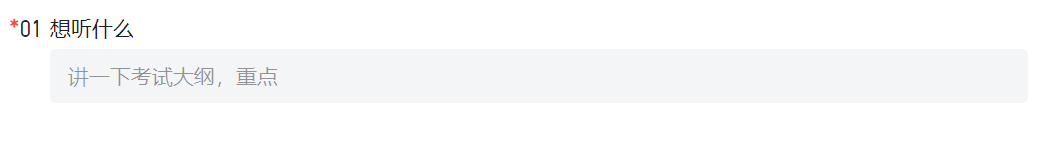
\includegraphics[width=1.0\textwidth]{figures/q3.png} % 替换为你的图片路径
    \end{center}
    可以参考 阅后即焚.pdf

\end{frame}

\begin{frame}{Q4}
    \begin{center}
        
\includegraphics[width=1.0\textwidth]{figures/q4.png} % 替换为你的图片路径
    \end{center}
    不是我出,无能为力。

\end{frame}

\begin{frame}{Q5}
    \begin{center}
        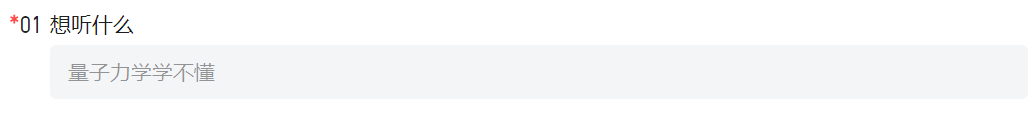
\includegraphics[width=1.0\textwidth]{figures/q5.png} % 替换为你的图片路径
    \end{center}
    俺也一样

\end{frame}

\begin{frame}{Q6}
    \begin{center}
        
\includegraphics[width=1.0\textwidth]{figures/q6.png} % 替换为你的图片路径
    \end{center}
    可以,不想来就不来。反正小班不用给分。

\end{frame}

\begin{frame}{Q7}
    \begin{center}
        
\includegraphics[width=1.0\textwidth]{figures/q7.png} % 替换为你的图片路径
    \end{center}
    我水平差,可能做不到...可以考虑去其他小班听听看。

\end{frame}


\end{document}
